\documentclass[10pt]{article}
\usepackage[T1]{fontenc}
\usepackage{lmodern,amsmath,amssymb,graphicx,hyperref}
\usepackage[margin=.74in]{geometry}
\setlength{\parindent}{0pt}\setlength{\parskip}{6pt}
\begin{document}
\begin{center}{\Large Public signed-Hankel construction}\\[4pt]
17 November 2026 --- local unsigned component evidence\end{center}
\textbf{Actual public objects.} For a finite support $S$ over a field $K$,
public branches $z$, and matrix size $m$, the actual existing module defines
\[
 \mu_j=\sum_{x\in S}\frac{z(x)x^j}{\prod_{t\in S\setminus\{x\}}(x-t)},
 \qquad H_{jk}=\mu_{j+k}\quad(0\le j,k<m).
\]
New source002 computes these through existing generic logged dot products,
using the actual support enumeration and public coefficients. It materializes
$(2m-1)_+$ moments in Vector-backed storage once; every row then reads those
stored entries. The resulting values equal the actual old $H b$.
Nonzero witness acceptance is equivalent to $\det H=0$. This is a verifier
construction; the branches and witness $b$ are not selected by it
[pcc:unverified].

\textbf{Exact emitted arithmetic.} Each multiplication count and each
addition count of the actual trace is
\[
 T=(2m-1)_+|S|+m^2,\qquad t_+=\max(t,0).
\]
This includes the chosen dot products, not public powers/denominators,
branch or input preparation, finite enumeration, field-bit arithmetic,
indexing, allocation, logging or control. At $m=0$, $T=0$: subtraction is truncated, as in the Lean natural-number statement. Empty-support cases also
remain in the formal statement [pcc:unverified].

For the literal realization with $q$ bits on each of two input words and
one output word of each binary field call, source003 constructs the call
and word-port index sets and obtains exactly $6qT$ ports. If $q\ge m$,
there are at least $6m^3$ declared ports. An explicit injective incidence
assignment of these ports into $E\times\{0,1\}$ would require
\[
 |E|\ge3qT,\qquad q\ge m\Longrightarrow |E|\ge3m^3.
\]
The incidence assignment is not constructed here. This is a conditional
screen of this literal realization, not an arbitrary-circuit or algorithm
runtime lower bound. Source structural edge count cannot be silently
replaced by ECDLP bit length; coefficient-description bits are separate.
Earlier arithmetic modulo $2^q$ is not automatically arithmetic in
$\mathbb F_p$ [pcc:unverified].

\textbf{Evidence map.} Public source002, build003, receipt001:
12 statements, PCC-20261117-ad0dcc. Source003, build004, receipt002:
16 including12 parent, PCC-20261117-9f2a9e. Source-level commands, versions,
input digests and failed attempts are retained in the pre-call records and
raw logs. All cited accepted builds exit0 without warnings and print only
standard foundational dependencies. Records are unsigned/default
\texttt{not\_covered}, outside shared Transport53/57 audit/fresh
[pcc:unverified].

\textbf{Requirement status.} Actual moment/row value and emitted-call binding:
local checked component. Full Boolean graph/field-bit preparation and
expected cost: open. Public sign/witness finder: open. The existing norm and
scalar bridge still have their explicit successful-input/label hypotheses.
\newpage
\begin{center}{\Large Rational list recovery: test the natural helper}\end{center}
\textbf{Literature first.} Beelen--H\o holdt--Nielsen--Wu (2013), Section III,
Theorem6, treats rational interpolation through partially projective points.
Its factor conclusion requires weighted degree strictly below multiplicity
times agreement. Multiple allowed ordinates are standard list-recovery input;
they are not themselves a novel method. The primary text and a separate
Rudra (2010) list-recovery lecture were read at the scopes recorded in
\texttt{literature-review-001.json}, unsigned PCC-20261117-4bcf3a
[pcc:unverified].

\textbf{A precise equality-boundary control.} Let $|S|=2a$ and consider the
natural homogeneous curve auxiliary
\[
 Q(X,Y,Z)=Y^2-f(X)Z^2.
\]
At any valid actual full norm $A^2-fB^2=C(c)G$, where $c\ne0$ and
$G=\prod_{x\in S}(X-x)$, substitution gives a nonzero polynomial.
For every natural $r$, source005 derives
\[
 Q(X,A,B)^r\ne0,\qquad
 \deg\bigl(Q(X,A,B)^r\bigr)=2ar.
\]
The actual public-input certificate endpoint supplies the norm from a
successful public Hankel determinant, rather than an arbitrary new norm
oracle. Thus powers of this fixed helper do not supply a strictly smaller
specialized root-degree certificate. This does not exclude independent
helpers or establish a full weighted-degree/multiplicity decoder theorem
[pcc:unverified].

\begin{center}
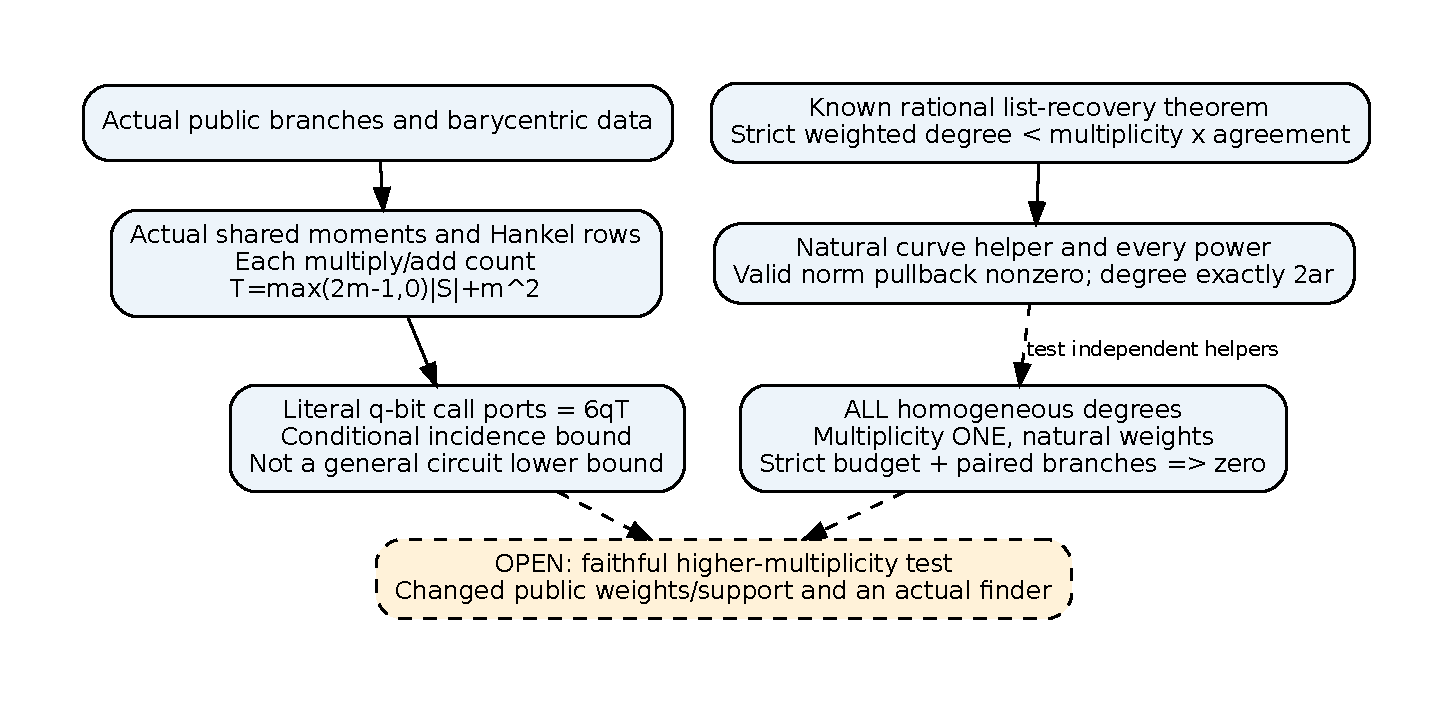
\includegraphics[width=.93\linewidth,height=3.35in,keepaspectratio]{dependencies-final-001.pdf}
\end{center}

\textbf{Scope.} Source005/build006/receipt003 adds8 statements to16 parent
statements; unsigned PCC-20261117-c7ea24. Earlier warning source004 and its
raw output remain exact. No decoder run or speed claim was made.
\newpage
\begin{center}{\Large All homogeneous degrees at multiplicity one}\end{center}
\textbf{Exact statement.} Fix $a\ge2$, $|S|=2a$, $2\ne0$ in $K$ and
$z(x)\ne0$ for every $x\in S$. For any $\ell\ge0$, write
\[
 Q(X,Y,Z)=\sum_{j=0}^{\ell}q_j(X)Y^jZ^{\ell-j}.
\]
Assume the literal strict coefficientwise budget at weights $(1,a,a-2)$:
\[
 \deg q_j+ja+(\ell-j)(a-2)<2a
 \quad\hbox{for every }j,
\]
where the degree of the zero polynomial is bottom. If
$Q(x,z(x),1)=Q(x,-z(x),1)=0$ for every support abscissa, then
\textbf{every coefficient $q_j$ is zero}. This is source009's
\texttt{strict\_symmetric\_interpolator\_zero}, with all exceptions and
quantifiers retained [pcc:unverified].

\textbf{Readable proof.} If $j\ge2$, the term $ja$ already uses at least
$2a$ weight, so strictness forces $q_j=0$. Every remaining coefficient has
degree less than $2a$. For $\ell\ge1$, the two branch equations reduce to
$q_0(x)+q_1(x)z(x)=0$ and $q_0(x)-q_1(x)z(x)=0$.
Since $2z(x)\ne0$, both coefficients vanish at all $2a$ distinct abscissas;
the existing polynomial root bound forces $q_0=q_1=0$. For $\ell=0$ the
single coefficient is handled directly. The Lean proof uses existing finite
sum splitting and nodal divisibility, with no new generic induction or
polynomial-division machinery [pcc:unverified].

The earlier all-quadratic case is source007/build008/receipt004,
PCC-20261117-7656f6. The arbitrary-degree extension is source009/build010/
receipt005, PCC-20261117-108594. Final source has29 statements including all
preceding local components, not29 new statements on top of them. All final
printed foundations are standard; local producer standing remains unsigned,
outside shared audit/fresh [pcc:unverified].

\textbf{What changes next.} Repeating this exact multiplicity-one symmetric
scheme on a different host cannot change the algebraic condition.
Higher or nonuniform multiplicity, different weights or public support
structure remain outside the result. First test a faithful higher-multiplicity
jet formulation; the saved induction sketch is unvalidated. A changed positive
candidate must actually select branches from public data, preserve a useful
nonzero target-scalar coefficient and charge all attempts, preparation,
field/bit work, recovery and retries. No general ECDLP existence or
nonexistence conclusion follows [pcc:unverified].

\textbf{Sources and preservation.}
\href{https://doi.org/10.1109/TIT.2013.2243800}{Beelen et al., 2013, Theorem6 (DOI)};
\href{https://cse.buffalo.edu/faculty/atri/courses/coding-theory/spr10/lectures/lect39.pdf}{Rudra, 2010, list-recovery lecture}.
This version explicitly displays truncated subtraction at $m=0$; the frozen earlier report is preserved.

Exact source002--009, maps001--005, receipts001--005, all failed or warning
sources and raw logs remain beside this report.

No paid, native, attack or scaling
campaign, timing result or canonical scoreboard change. Original immutable
reports and ledger history remain exact; publication is still subject to the
protected provenance blocker. Next action: \texttt{PROTOCOL-001.md}.
\end{document}
